% !TeX root = ./0-Tesis-de-maestria-JLBG.tex
En este capítulo se muestra el enfoque de la electrodinámica clásica empleado para describir la interacción de un electrón rápido y una nanopartícula (NP) esférica. En partícular, se estudia la interacción a partir del momento lineal transferido del electrón a la NP. Un trabajo reciente de García de Abajo \cite{deabajo2021optical} justifica que bajo la condiciones establecidas en la introducción, no es necesaria una descripción cuántica del fenómeno.

Las siguientes ecuaciones se encuentran en el sistema $\cgs{\text{cgs}}$ Internacional; es decir, se proporciona en color \textbf{negro} la ecuación en sistema Internacional, y entre paréntesis y resaltado con color $\cgs{\text{magenta}}$ el factor necesario para expresar la ecuación en el sistema cgs. Por ejemplo, la fuerza entre dos cargas puntuales $q_1$ y $q_2$ separadas una distancia $r$ se escribiría como
\begin{equation}
\vv{F} = \cgs{4\pi\epsilon_0}\frac{1}{4\pi\epsilon_0} \frac{q_1 q_2}{r^2} \hat{r}
\end{equation}

\subsection{Conservación del momento angular en electrodinámica}
Trabajando en el sistema $\cgs{\text{cgs}}$ internacional, las ecuaciones de Maxwell se escriben como \cite{jackson}
%%%%%%%%%%%%%%%% ECUACIONES DE MAXWELL
\begin{align}
\nabla\cdot\vv{E} =& \cgs{4\pi\epsilon_0}\frac{\rho_{\text{tot}}}{\epsilon_0}, \qquad \qquad \nabla\times\vv{E}=-\cgs{\frac{1}{c}}\frac{\partial\vv{B}}{\partial t}, \nonumber \\
\nabla\cdot\vv{B} =& 0, \qquad \qquad \qquad \qquad \nabla\times\vv{B}=\cgs{\frac{4\pi}{\mu_0 c}}\mu_0\vv{J}_{\text{tot}}+\cgs{c}\frac{1}{c^2}\frac{\partial\vv{E}}{\partial t},
\label{eq: Maxwell equations}
\end{align}
y pueden ser reescritas en términos de los potenciales $\phi$ y $\vv{A}$ como \cite{jackson}
%%%%%%%%%%%%%%% ECUACIONES DE ONDA PARA LOS POTENCIALES
\begin{align}
\var{\nabla^2 -\frac{1}{c^2}\frac{\partial}{\partial t}}\phi\vars =& - \cgs{4\pi\epsilon_0} \frac{\rho_{\text{tot}}}{\epsilon_0}\vars, \label{eq: scalar potential}\\
\var{\nabla^2 -\frac{1}{c^2}\frac{\partial}{\partial t}}\vv{A}\vars =& - \cgs{\frac{4\pi}{\mu_0 c}}\mu_0 \vv{J}_{\text{tot}}\vars,\label{eq: vector potential}
\end{align}
trabajando en la norma de Lorentz, donde se satisface que $\nabla\cdot\vv{A}+\cgs{1/c}\partial_t \phi =0$, y los campos electromagnéticos se escriben en términos de los potenciales como
%%%%%%%%%%%%%%% ECUACIONES DE CAMPO EN TÉRMINOS DE LOS POTENCIALES
\begin{align}
\vv{E}\vars =& \, -\nabla\phi\vars - \cgs{\frac{1}{c}}\frac{\partial}{\partial t}\vv{A}\vars, \label{eq: E field potentials}\\
\vv{B}\vars =& \, \nabla\times\vv{A}\vars. \label{eq: B field potentials}
\end{align}

Partiendo de la expresión para la conservación del momento lineal \cite{jackson}
%%%%%%%%%%%%%%% CONSERVACIÓN DEL MOMENTO LINEAL EN ELECTRODINÁMICA
\begin{equation}
\frac{\partial}{\partial t} \Var{\vv{p}^{\rm mec}\var{\vv{r},t}+\vv{p}^{\rm em}\var{\vv{r},t}} = \nabla \cdot \tensa{T}\var{\vv{r},t},
\label{eq: cons momento lineal}
\end{equation}
donde $\vv{p}^{\rm mec}\var{\vv{r},t}$ es la densidad de momento lineal mecánico, $\vv{p}^{\rm em}\var{\vv{r},t}$ es la densdad de momento lineal electromagnético
%%%%%%%%%%%%%%% MOMENTO LINEAL ELECTROMAGNÉTICO
\begin{equation}
\vv{p}^{\rm em}\vars = \cgs{\frac{c}{4\pi}}\frac{1}{c^2}\vv{E}\vars\times\vv{B}\vars
\end{equation}
y $\tensa{T}\var{\vv{r},t}$ es el tensor de esfuerzos de Maxwell dado por \cite{jackson}
%%%%%%%%%%%%%%% TENSOR DE ESFUERZOS DE MAXWELL
\begin{equation}
T_{ij}\var{\vv{r},t}= \frac{\epsilon_0}{\cgs{4\pi\epsilon_0}} \Var{E_i\var{\vv{r},t}E_j\var{\vv{r},t} -\frac{\delta_{ij}}{2}E^2\vars} +  \frac{\mu_0}{\cgs{4\pi\mu_0}} \Var{ H_i\var{\vv{r},t}H_j\var{\vv{r},t} -\frac{\delta_{ij}}{2}H^2\vars } ,
\end{equation}
donde se ha asumido que $T_{ij}\var{\vv{r},t}$ es la entrada $ij$ de $\tensa{T}\var{\vv{r},t}$, $\epsilon_0$ y $\mu_0$ son la permitividad y permeabilidad del vacío respectivamente, $E_i\var{\vv{r},t}$ es la $i$-ésima componente del campo eléctrico $\vv{E}\var{\vv{r},t}$, $H_i\var{\vv{r},t}$ es la $i$-ésima componente del campo magnético $\vv{H}\var{\vv{r},t}$ y $\delta_{ij}$ es la delta de Kronecker. 

Partiendo de la Ec. \eqref{eq: cons momento lineal}, la conservación de momento angular se puede escribir como
\begin{equation}
\frac{\partial}{\partial t} \var{\vvb{\ell}^{\rm \, mec}\var{\vv{r},t}+\vvb{\ell}^{\rm \, em}\var{\vv{r},t}} = \vv{r}\times\nabla \cdot \tensa{T}\var{\vv{r},t},
\end{equation}
donde $\vvb{\ell}^{\rm \, mec}\var{\vv{r},t}=\vv{r}\times\vv{p}^{\rm mec}\var{\vv{r},t}$ y $\vvb{\ell}^{\rm \, em}\var{\vv{r},t}=\vv{r}\times\vv{p}^{\rm em}\var{\vv{r},t}$ son las densidades volumétricas de momento angular mecánico y electromagnético respectivamente.

Si se define $\tensa{M}\var{\vv{r},t}=\vv{r}\times\tensa{T}\var{\vv{r},t}$ \textemdash o usando notación de índices y convención de suma de Einstein $M_{jk}\var{\vv{r},t}=\epsilon_{j}^{\,\,\,\, li} r_l T_{ik}\var{\vv{r},t}$\textemdash y se calcula la divergencia de $\tensa{M}$, se obtiene 
\begin{align}
\var{\nabla\cdot\tensa{M}}_{j} =& \,\delta^{nk} \partial_n M_{jk} = \delta^{nk} \partial_n \epsilon_{j}^{\,\,\,\, li} r_l T_{ik} =\delta^{nk}\epsilon_{j}^{\,\,\,\, li}\partial_n r_l T_{ik}, \nonumber \\
								=& \,\delta^{nk}\epsilon_{j}^{\,\,\,\, li}\var{\delta_{nl} T_{ik} + r_l \partial_n T_{ik}} =\delta^{nk}\epsilon_{j}^{\,\,\,\, li}r_l\partial_n T_{ik}, \nonumber \\
								=& \,\delta^{nk} \epsilon_{j}^{\,\,\,\, li} r_l \partial_n T_{ik} = \epsilon_{j}^{\,\,\,\, li} r_l \partial^k T_{ik} = \epsilon_{j}^{\,\,\,\, li} r_l \var{\nabla\cdot\tensa{T}}_i, \nonumber \\
\var{\nabla\cdot\tensa{M}}_{j} =& \var{\vv{r}\times \nabla\cdot\tensa{T}}_j,
\end{align}
donde se ha usado $\delta^{nk}\delta_{nl}\,\epsilon_{j}^{\,\,\,\, li}T_{ik} = \epsilon_{j}^{\,\,\,\, ni}T_{in} = 0$, porque el tensor de esfuerzos de Maxwell es simétrico $\var{T_{in}=T_{ni}}$ y el símbolo de Levi-Civita es antisimétirco $\var{\epsilon_{j}^{\,\,\,\, ni}=-\epsilon_{j}^{\,\,\,\, in}}$.

A partir de este resultado se puede escribir la conservación del momento angular como
\begin{equation}
\frac{\partial}{\partial t} \var{\vvb{\ell}^{\rm \, mec}\var{\vv{r},t}+\vvb{\ell}^{\rm \, em}\var{\vv{r},t}} = \nabla \cdot \tensa{M}\var{\vv{r},t},
\label{eq: cons momento angular}
\end{equation}
qe es una ecuación local. Para escribir la conservación del momento angular de forma global, se debe integrar la Ec. \eqref{eq: cons momento angular} sobre un volumen $V$ delimitado por una superficie $S$ de la siguiente manera
\begin{align}
\frac{d}{dt}\var{\vv{L}^{\rm mec}\var{t}+\vv{L}^{\rm em}\var{t}} =& \int_V \nabla\cdot\tensa{M}\var{\vv{r},t} \, dV, \nonumber \\
\frac{d}{dt}\var{\vv{L}^{\rm mec}\var{t}+\vv{L}^{\rm em}\var{t}} =& \oint_S \tensa{M}\var{\vv{r},t} \, \cdot d\vv{S},
\label{eq: cons momento angular global}
\end{align}
donde se ha usado el teorema de la divergencia en la última igualdad, y se han definido 
\begin{equation}
\vv{L}^{\rm mec}\var{t} = \int_V \vvb{\ell}^{\, \rm mec}\var{\vv{r},t}\, dV, \qquad\qquad \text{y} \qquad\qquad \vv{L}^{\rm em}\var{t} = \int_V \vvb{\ell}^{\, \rm em}\var{\vv{r},t}\, dV.
\end{equation}

\begin{figure}[h!]
\centering
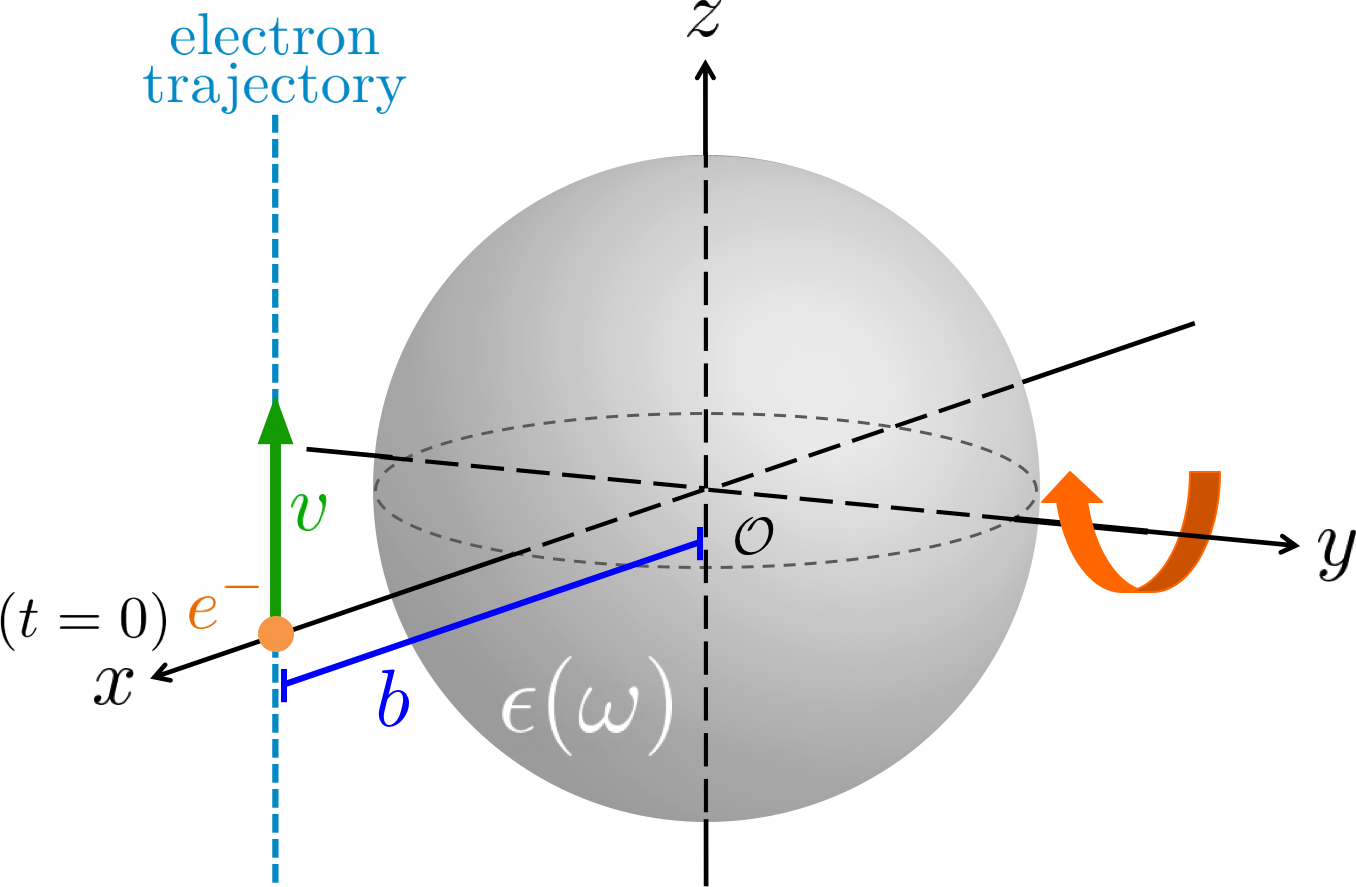
\includegraphics[width=0.5\linewidth]{system.pdf}
\caption{\label{fig: system}Nanopartícula caracterizada por una respuesta dieléctrica homogénea $\epsilon\var{\w}$ centrada en el origen, junto a la trayectoria del electrón colocada en $\vv{r}=(0,b,vt)$}
\end{figure}

Se define el sistema de estudio como el de una NP caracterizada por una respuesta dieléctrica homogénea $\epsilon\var{\w}$ centrada en el origen, interactuando con un electrón cuya trayectoria se describe a través de $\vv{r}=(0,b,vt)$, como se muestra en la Fig. \ref{fig: system}. Para calcular la transferencia de momento angular del electrón a la NP ($\Delta \vv{L}$) se integra la Ec. \eqref{eq: cons momento angular global} en el tiempo de la siguiente manera
\begin{equation}
\Delta\vv{L} = \intt{\frac{d}{dt}\vv{L}^{\rm mec}\var{t}} = \intt{\intS{\tensa{M}\var{\vv{r},t}}} - \Delta\vv{L}^{\rm em},
\end{equation}
donde 
\begin{equation}
\Delta\vv{L}^{\rm em}=\intt{\frac{d}{dt}\vv{L}^{\rm em}} = \vv{L}^{\rm em}(t\to\infty)-\vv{L}^{\rm em}(t\to-\infty),
\end{equation}
y
\begin{equation}
\vv{L}^{\rm em}(t\to\pm\infty) = \epsilon_0 \mu_0  \intV{\vv{r}\times\Var{\vv{E}\var{t\to\pm\infty}\times\vv{H}\var{t\to\pm\infty}}},
\label{eq: Lem}
\end{equation}
donde este último término, para el sistema de estudio de este trabajo, es nulo porque en el tiempo $t\to -\infty$ el electrón se encuentra infinitamente lejos y no ha interactuado con la NP, por lo que los campos electromagnéticos son nulos \textemdash$\vv{E}\var{t\to-\infty}=\vv{0}$ y $\vv{H}\var{t\to-\infty}=\vv{0}$\textemdash; posteriormente, para cuando $t\to\infty$, el electrón se encontrará infinitamente lejos de la NP pero ya habrá interactuado con ella, por lo que se habrán inducido distribuciones de cargas y corrientes eléctricas dentro de la NP, que habrán desaparecido para cuando $t\to\infty$ debido a procesos disipativos. Por tanto $\vv{L}^{\rm em}\var{t\to\pm\infty}=0$.

Entonces
\begin{equation}
\Delta\vv{L} = \intt{\intS{\tensa{M}\var{\vv{r},t}}},
\end{equation}
o usando notación de índices
\begin{equation}
\Delta L_i =  \intt{\oint_S \epsilon_{i}^{\,\,\,\, lj} r_l T_{jk}\var{\vv{r},t} n^k\,dS},
\label{eq: angular momentum transfer index notation}
\end{equation}
donde $n_i$ es la $i$-ésima componente del vector normal a la superficie de S.

Como la función dieléctrica $\epsilon\var{\w}$ se presenta usualmente en términos de la frecuencia, resulta conveniente expresar a los campos electromagnéticos en términos de $\w$. Mediante la transformada de Fourier temporal se pueden expresar los campos electromagnéticos en función de la frecuencia, de la sigueinte manera
\begin{equation}
\vv{F}(\w) = \intt{\vv{F}(t)\,{\rm e}^{{\rm i} \w t}} \qquad \text{y} \qquad \vv{F}(t) = \frac{1}{2\pi}\intw{\vv{F}(\w)\,{\rm e}^{-{\rm i} \w t}}
\end{equation}
donde $\vv{F}\in \{ \vv{B}, \vv{H}\}$ y para que $\vv{F}(t)$ sea una función de variable real se debe cumplir que $\vv{F}(\w)^{*}=\vv{F}(-w)$ con la convención de exprezar al complejo conjugado de un número $z$ como $z^{*}$. Además, para calcular la transferencia de momento angular a través de la Ec. \eqref{eq: angular momentum transfer index notation} es importante notar que la dependencia en el tiempo está contenida únicamente en el tensor de esfuerzos de Maxwell $\tensa{T}\var{\vv{r},t}$. De esta forma se puede reescribir la integrar en el tiempo de la siguiente manera
\begin{align}
\intt{E_i\vars E_j \vars} =& \intt{\Var{\frac{1}{2\pi}\intw{E_i\varsw \,{\rm e}^{-{\rm i} \w t} }} \Var{\frac{1}{2\pi}\intw{E_j\var{\vv{r},\w^{\prime}} \,{\rm e}^{-{\rm i} \w^{\prime} t} }^{\prime}} },\nonumber\\
=&\frac{1}{2\pi} \intw{\intw{\Var{\frac{1}{2\pi}\intt{{\rm e}^{-{\rm i}\var{\w+\w^{\prime}} t}}} E_i \varsw E_j\var{\vv{r},\w^{\prime}}}}^{\prime},\nonumber\\
=&\frac{1}{2\pi}\intw{\intw{\delta\var{\w+\w^{\prime}} E_i \varsw E_j\var{\vv{r},\w^{\prime}} }}^{\prime},\nonumber\\
=&\frac{1}{2\pi}\intw{ E_i \varsw E_j\var{\vv{r},-\w} }=\frac{1}{2\pi}\intw{ E_i \varsw E_j^{*}\varsw },\nonumber\\
=&\frac{1}{\pi}\intwo{{\rm Re}\Var{E_i\varsw E_j^{*}\varsw}}
\end{align}
y se puede realizar el proceso análogo para las componentes del campo $\vv{H}$.

De esta manera se puede reescribir la Ec. \eqref{eq: angular momentum transfer index notation} como
\begin{equation}
\Delta L_i = \frac{1}{\pi} \intwo{\oint_S \epsilon_{i}^{\,\,\,\, lj} r_l \mathcal{T}_{jk}\varsw n^k\,dS},
\label{eq: angular momentum transfer index notation freq domain}
\end{equation}
donde se ha definido 
\begin{align}
\tensa{\mathcal{T}}\varsw =& \,{\rm Re}\Bigg[\frac{\epsilon_0}{\cgs{4\pi\epsilon_0}} \vv{E} \varsw \vv{E}^{*}\varsw-\frac{\epsilon_0}{\cgs{4\pi\epsilon_0}} \frac{\tensa{I}}{2} \vv{E} \varsw\cdot\vv{E}_j^{*}\varsw \nonumber \\
& + \frac{\mu_0}{\cgs{4\pi\mu_0}} \vv{H}_i \varsw \vv{H}_j^{*}\varsw- \frac{\mu_0}{\cgs{4\pi\mu_0}} \frac{\tensa{I}}{2}  \vv{H} \varsw\cdot\vv{H}^{*}\vars \Bigg],
\end{align}
donde $\tensa{I}$ es el tensor identidad de rango 2. De esta forma se puede definir finalmente la <<densidad espectral>> de momento angular 
\begin{equation}
\mathcal{L}_i\var{\w} = \frac{1}{\pi} \oint_S \epsilon_{i}^{\,\,\,\, lj} r_l \mathcal{T}_{jk}\varsw n^k\,dS.
\end{equation}
y calcular la transferencia de momento angular a través de 
\begin{equation}
\Delta \vv{L} = \intwo{\vv{\mathcal{L}}\var{\w}}.
\label{eq: densidad espectral momento angular}
\end{equation}

Resulta adecuado separar la contribución eléctrica de la magnética de la densidad espectral de la Ec.\eqref{eq: densidad espectral momento angular}. Para realizar esto se debe separar
\begin{equation}
\tensa{\mathcal{T}}\varsw = \tensE{\mathcal{T}}\varsw +\tensH{\mathcal{T}}\varsw 
\end{equation}
con 
\begin{align}
\tensE{\mathcal{T}}=& \frac{\epsilon_0}{\cgs{4\pi\epsilon_0}} \re{\vv{E}\varsw \vv{E}^{*}\varsw - \frac{\tensa{I}}{2} \vv{E}\varsw\cdot\vv{E}^{*}\varsw},\\
\tensH{\mathcal{T}}=& \frac{\mu_0}{\cgs{4\pi\mu_0}} \re{\vv{H}\varsw \vv{H}^{*}\varsw - \frac{\tensa{I}}{2} \vv{H}\varsw\cdot\vv{H}^{*}\varsw}.
\end{align}

Si se elige una esfera como superficie de integración, y se denota a $R$ como el radio de la superficie de integración esférica $S$ y a $\hat{r}_i$ como la $i$-ésima componente del vector unitario radial, es posible expresar a $\mathcal{L}_i \var{\w}$ de la siguiente manera
\begin{equation}
\mathcal{L}_i\var{\w} = \frac{R^2}{\pi} \int_0^{4\pi} \Var{\epsilon_{i}^{\,\,\,\, lj} r_l \mathcal{T}^{\, \rm E}_{jk}\varsw n^k + \epsilon_{i}^{\,\,\,\, lj} r_l \mathcal{T}^{\, \rm H}_{jk}\varsw n^k}\,d\Omega,
\label{Eq: complete spectral component of AMT with spherical symmetry}
\end{equation}
donde únicamente falta integral en el ángulo sólido $\Omega$. Se puede separar la contribución eléctrica de la magnética en la Ec. \eqref{Eq: complete spectral component of AMT with spherical symmetry} de la siguiente manera
\begin{align}
\mathcal{L}_i^{\rm E}\var{\w} = \frac{R^2}{\pi} \int_0^{4\pi} \Var{\epsilon_{i}^{\,\,\,\, lj} r_l \mathcal{T}^{\,\rm E}_{jk}\varsw n^k}\,d\Omega, \\
\mathcal{L}_i^{\rm H}\var{\w} = \frac{R^2}{\pi} \int_0^{4\pi} \Var{\epsilon_{i}^{\,\,\,\, lj} r_l \mathcal{T}^{\,\rm H}_{jk}\varsw n^k}\,d\Omega.
\end{align}

Se pueden separar a los campos electromagnéticos $\vv{E}$ y $\vv{H}$ en sus contribuciones de campo externo (ext) y campo esparcido (scat) como 
\begin{equation}
\vv{E} = \EE{ext} + \EE{scat}, \qquad\qquad \text{y} \qquad\qquad \vv{H} = \HH{ext} + \HH{scat},
\end{equation}
donde $\EE{ext}$ y $\HH{ext}$ son los campos electromagnéticos externos \textemdash es decir, los producidos por el electrón\textemdash, y $\EE{scat}$ y $\HH{scat}$ son los campos esparcidos por la nanopartícula (NP). Mediante esta separación se puede reescribir la componente eléctrica del tensor de esfuerzos como
\begin{align}
\tensE{\mathcal{T}}=&\,\frac{\epsilon_0}{\cgs{4\pi\epsilon_0}} \re{ \var{\EE{ext}+\EE{scat}}\var{\EE{ext}^{*}+\EE{scat}^{*}}-\frac{\tensa{I}}{2}\var{\EE{ext}+\EE{scat}}\cdot\var{\EE{ext}^{*}+\EE{scat}^{*}} },\nonumber \\
=& \, \frac{\epsilon_0}{\cgs{4\pi\epsilon_0}} {\rm Re} \Bigg[\var{\EE{scat}\EE{scat}^{*}+\EE{scat}\EE{ext}^{*}+\EE{ext}\EE{scat}^{*}+\EE{ext}\EE{ext}^{*}}\nonumber \\
&-\frac{\tensa{I}}{2}\var{\EE{scat}\cdot\EE{scat}^{*}+\EE{scat}\cdot\EE{ext}^{*}+\EE{ext}\cdot\EE{scat}^{*}+\EE{ext}\cdot\EE{ext}^{*}} \Bigg].
\label{eq: tensor de esfuerzos inicio}
\end{align}
Por medio de esta separación se puede escribir la componente eléctrica del tensor de esfuerzos como
\begin{equation}
\tensE{\mathcal{T}}=\tensE{\mathcal{T}}_{\rm ss}+\tensE{\mathcal{T}}_{\rm int}+\tensE{\mathcal{T}}_{\rm ee}
\end{equation}
en donde

\begin{align}
\tensE{\mathcal{T}}_{\rm ss} =& \frac{\epsilon_0}{\cgs{4\pi\epsilon_0}} \re{\EE{scat}\EE{scat}^{*}-\frac{\tensa{I}}{2}\EE{scat}\cdot\EE{scat}^{*}},\\
\tensE{\mathcal{T}}_{\rm ee} =& \frac{\epsilon_0}{\cgs{4\pi\epsilon_0}} \re{\EE{ext}\EE{ext}^{*}-\frac{\tensa{I}}{2}\EE{ext}\cdot\EE{ext}^{*}}, \\
&\tensE{\mathcal{T}}_{\rm int} = \tensE{\mathcal{T}}_{\rm se} + \tensE{\mathcal{T}}_{\rm es}
\end{align}
con

\begin{align}
\tensE{\mathcal{T}}_{\rm es} =& \frac{\epsilon_0}{\cgs{4\pi\epsilon_0}} \re{\EE{ext}\EE{scat}^{*}-\frac{\tensa{I}}{2}\EE{ext}\cdot\EE{scat}^{*}},\\
\tensE{\mathcal{T}}_{\rm se} =& \frac{\epsilon_0}{\cgs{4\pi\epsilon_0}} \re{\EE{scat}\EE{ext}^{*}-\frac{\tensa{I}}{2}\EE{scat}\cdot\EE{ext}^{*}}.
\label{eq: tensor de esfuerzos final}
\end{align}
Análogamente al hacer la sustitución $\epsilon_0 \to \mu_0$ y $\vv{E}\to\vv{H}$ en las Ecs. \eqref{eq: tensor de esfuerzos inicio} a \eqref{eq: tensor de esfuerzos final}, se obtiene las contribuciones magnéticas al tensor $\tensa{\mathcal{T}}$, denotadas por $\hspace{-0.6 em}\tensH{\mathcal{T}}_{\rm ij}$ donde $\rm ij$ pueden tomar los valores \{$\rm e$, $\rm s$\}.

Se puede interpretar a $\tensa{\mathcal{T}}_{\rm int}$ como la componente que está relacionada con la interacción del campo electromagnético del electrón con las cargas y corrientes inducidas en la NP. En el caso en que no exista NP, nada altera el movimiento del electrón, por lo que no pierde ni cede energía, momento lineal ni momento angular ($\Delta L = 0$) \cite{castellanos2021phdthesis}. Al no existir NP, los campos electromagnéticos esparcidos serían nulos, por lo que la única contribución al momento angular proviene de la componente $\tensa{\mathcal{T}}_{\rm ee}$. Por tanto, de manera general, se concluye que la contribución al momento angular transferido debido a $\tensa{\mathcal{T}}_{\rm ee}$ es nula, por lo que no será considerada en los cálculos subsecuentes. También vale la pena mencionar que la componente $\tensa{\mathcal{T}}_{\rm ss}$, al depender únicamente de los campos electromagnéticos esparcidos por la NP, está relacionada con la interacción de la NP consigo misma, referida por algunos autores como reacción de radiación \cite{jackson}.  

En la siguiente sección se presentan las expresiones analíticas de los campos electromagnéticos externos (producidos por el electrón) y de los esparcidos por la NP, para poder integrarlos dentro de la Ec. \eqref{Eq: complete spectral component of AMT with spherical symmetry}.
%
% 	TRANSFERENCIA DE MOMENTO ANGULAR DE UN ELECTRÓN RÁPIDO A UNA NANOPARTÍCULA ESFÉRICA
%
\subsection{Transferencia de momento angular de un electrón rápido a una nanopartícula}
El campo electromagnético externo producido por un electrón rápido, considerado como una partícula puntual de carga $q=-e$, viajando a velocidad $\vv{v}$ constante a lo largo del eje z [ver Fig. \ref{fig: system}], se puede obtener mediante una transformación de Lorentz de un sistema de referencia en el que el electrón se encuentra en reposo, a un sistema de referencia en el que el electrón que se mueve a velocidad constante $\vv{v}$, obteniendo \cite{jackson}
\begin{align}
\EE{ext}\vars =& \cgs{4\pi\epsilon_0}\frac{-e}{4\pi\epsilon_0}\frac{\gamma \Var{\vv{R}+(z-vt)\hat{z}}}{\Var{R^2+\gamma^2(z-vt)^2}^{3/2}}, \label{eq: Eext}\\
\HH{ext}\vars =& \cgs{4\pi}\frac{-e}{4\pi}\frac{\gamma \, \vv{v}\times\vv{R}}{\Var{R^2+\gamma^2(z-vt)^2}^{3/2}}, \label{eq: Hext}
\end{align}
en donde $\gamma = \var{1-\beta^2}^{-1/2}$, $\beta = v/c$, $\vv{R}=(x-b)\hat{x}+y\hat{y}$, $R = \sqrt{(x-b)^2+y^2}$ y $\vv{v}\times\vv{R}=v\Var{(x-b)\hat{y}-y\hat{x}}$. Se pueden calcular los campos electromagnéticos externos en función de la frecuencia mediante una transformada de Fourier de las Ecs. \eqref{eq: Eext} y \eqref{eq: Hext} que se expresan como \cite{maciel2019electromagnetic}
\begin{align}
\EE{ext}\varsw = &\cgs{4\pi\epsilon_0}\frac{-e}{4\pi\epsilon_0}  \frac{2\w}{v^2 \gamma} \rme^{\rmi \w (z/v)} \left\{ {\rm sign}(\w) K_1\wR\hat{R} - \frac{\rmi}{\gamma}K_0\wR \hat{z}\right\},\\
&\HH{ext}\varsw = \cgs{4\pi}\frac{-e}{4\pi}\frac{2e}{v c \gamma} \abs{\omega} {\rm e}^{{\rm i}\omega z /v} K_1\wR \hat{v}\times\hat{R},
\end{align}
que son expresiones cerradas con simetría cilíndrica. Como también se buscan los campos esparcidos por la NP, que tienen simetría esférica, conviene expresar a los campos electromagnéticos del electrón mediante una solución con simetría esférica. 

El campo eléctrico producido por el electrón se puede obtener mediante la función de Green dependiente del tiempo \cite{maciel2019electromagnetic}  
\begin{equation}
\EE{ext}\varsw = e\var{\nabla-\rmi \frac{k\vv{v}}{c}} \intt{\rme^{\rmi \w t} G_0 \var{\vv{r}-\vv{r}_t}},
\label{eq: E field Green function}
\end{equation}
donde la función de Green $G_0 \var{\vv{r}-\vv{r}_t}$ está dada por 
\begin{equation}
G_0 \var{\vv{r}-\vv{r}_t} = \frac{\cgs{4\pi\epsilon_0}}{4\pi\epsilon_0}\frac{\rme^{\rmi k \abs{\vv{r}-\vv{r}_t}}}{\abs{\vv{r}-\vv{r}_t}},
\end{equation}
con $k = \w/c$ el número de onda en el vacío, $\vv{r}_t=\vv{r}_0+\vv{v}t$ la posición del electrón al tiempo $t$. Al expandir la función de Green en base esférica se obtiene \cite{de1999relativistic}
\begin{equation}
G_0(\vv{r}-\vv{r}_t) = \frac{\cgs{4\pi\epsilon_0}}{\epsilon_0} k \sum_{\ell = 0}^{\infty} \sum_{m=-\ell}^{\ell} j_{\ell}(kr) h_{\ell}^{+}(k r_t) Y_{\ell, m}(\Omega_r) Y_{\ell, m}(\Omega_{r_t})^{*},
\label{eq: Green function spherical base}
\end{equation}
donde $h_{\ell}^{+}(x) = \rmi h_{\ell}^{1}(x)$ es la función de Hankel esférica de orden $\ell$ \citep{Abramowitz}. Sustituyendo la Ec. \eqref{eq: Green function spherical base} en la Ec. \eqref{eq: E field Green function}, se obtiene
\begin{equation}
\EE{ext}\vars = \var{\nabla-\rmi \frac{k\vv{v}}{c}} \sum_{\ell = 0}^{\infty} \sum_{m=-\ell}^{\ell} j_{\ell}(kr) Y_{\ell, m}(\Omega_{r})\phi_{\ell, m}
\end{equation}
donde 
\begin{equation}
\phi_{\ell, m} = \frac{\cgs{4\pi\epsilon_0}}{\epsilon_0} k \intt{e^{i \omega t} h_{\ell}^{+}(k r_{t}) Y_{\ell, m}^{*}(\Omega_{r_t}) }.
\label{Eq: GdA phi coeffs}
\end{equation}

En el \hyperref[AppendixScalarPotentials]{Apéndice A} se muestran los detalles del cálculo de la Ec. \eqref{Eq: GdA phi coeffs}. Como se muestra también en el \hyperref[AppendixScalarPotentials]{Apéndice A}, es posible obtener expresiones para el campo electromagnético externo en representación multipolar esférica:



De este modo, sustituyendo la Ec. (\ref{Tsymmetry}) en la Ec. (\ref{indexangularmomentumconservation}) se obtiene que
%
%-------conservation of angular momentum 2----------
\begin{empheq}[box=\mymath]{equation}
	\frac{\partial}{\partial r_j}M_{kj}
	=
	\frac{\partial}{\partial t}\left( \ell^\text{mec}_k + \ell^\text{em}_k  \right),
	\label{angularmomentumconservation2}
\end{empheq}
%-------------------------------------------------
%
en donde
%
%-------Tensor M----------
\begin{equation}
M_{kj}
=
\epsilon_{kli}r_lT_{ij}
\label{tensorM}.
\end{equation}
%-------------------------------------------------
%
La Ec. (\ref{angularmomentumconservation2}) es la forma local de la conservación del momento angular. Integrando la Ec. (\ref{angularmomentumconservation2}) en el volumen interior $V$ de alguna superficie diferenciable $S$, estática y cerrada, y utilizando el teorema de la divergencia, se encuentra que la forma global de la conservación del momento angular es \cite{Good}:
%
\begin{mybox}{\centering  Conservación del momento angular en electrodinámica}
	\begin{equation}
	\oint_S \tensb{M} \cdot d\vv{a}
	=
	\frac{d}{dt}\left( \vv{L}^\text{mec} + \vv{L}^\text{em}  \right)
	\label{angularmomentumconservation3}
	\end{equation}
\end{mybox}	
%
% 

\noindent
en donde
%
%-------Lmech----------
\begin{equation}
\vv{L}^\text{mec}
=
\int_V \vvb{\ell}^\text{ mec} dV
\label{Lmech}
\end{equation}
%-------------------------------------------------
%
y
%
%-------Lem----------
\begin{equation}
\vv{L}^\text{em}
=
\int_V \vvb{\ell}^\text{ em} dV
\label{Lem}.
\end{equation}
%-------------------------------------------------
%
%*******************************************************
%*******************************************************


